\chapter{Getting started\label{sec:install}}

Here is where you find basic information for obtaining and installing the FLEXWIN package.
For details of how to tune the algorithm to your seismograms, see chapter~\ref{sec:tuning}.

\section{System requirements}
In order to install and run, FLEXWIN requires:
\begin{itemize}
\item UNIX operating system (Linux, Solaris, MacOS \ldots)
\item GNU make
\item a fortran compiler (gfortran, ifort, etc...) 
\item other packages : SAC (Seismic Analysis Code, available from IRIS); GMT (Generic Mapping Tools) for the plotting scripts
\end{itemize}

FLEXWIN requires the following libraries external to the package in order to
compile and run: {\tt libsacio.a} and {\tt libsac.a}. Both libraries
are distributed by IRIS as part of the SAC package (version 101.2 and above).
The IRIS download site (as of 30-March-2009) is here:
\url{http://www.iris.edu/software/sac/sac.request.htm}.
(To check your version, type sac.)


\section{Obtaining the code}

The code is available as a gzipped tarball from CIG (Computational Infrastructure for Geodynamics, \url{http://www.geodynamics.org}). The tarball is unpacked by typing {\tt tar xvzf flexwin.tgz}.

The package contains the flexwin code and documentation, as well as a set of
test data, examples of user files for different scenarios, and a set of utility
scripts that may be useful for running flexwin on large datasets.


\section{Compilation}

If your compiler of choice is gfortran, then you should be able to use the
{\tt make\_gfortran} makefiles with only minor modifications (notably you may need to
change the search path for the {\tt libsacio.a} library).  If you prefer another
compiler, you should modify the OPT and FC lines in the makefiles accordingly. We tested the code using gfortran version 4.1.2
(To check your version, type {\tt gfortran --version}.)  

{\bf Important note}: All the code is compiled with the -m32 option, which makes
32bit binaries.  This option is currently required to enable compatibility with
SAC.  Future versions of the SAC distribution may no longer require this
compatibility flag.

Steps to compile the flexwin package:
\begin{enumerate}
\item Compile {\tt libtau.a} and create {\tt iasp91.hed} and {\tt iasp91.tbl}.  In the {\tt flexwin/ttimes\_mod} directory type: {\tt make -f make\_gfortran}.  This will compile {\tt libtau.a}, and two programs, {\tt remodl} and {\tt setbrn}.  The makefile will also run {\tt remodl} and {\tt setbrn} to create the {\tt iasp91.hed}and {\tt iasp91.tbl} files.  You should then type {\tt make -f make\_gfortran install} to install the iasp91 files.
\item Compile flexwin.  Edit the {\tt make\_gfortran} file in the flexwin root directory to ensure the {\tt SACLIBDIR} environment variable points to the location of your SAC libraries (by default {\tt \$SACHOME/lib}).  Then type {\tt make -f make\_gfortran}.
\end{enumerate}

You should end up with the {\tt flexwin} executable.  The program requires the {\tt iasp91.hed} and {\tt iasp91.tbl} files (or symbolic links to them) to be present in the directory from which the code is launched. 


\section{Running the Test case}

You should test your compiled code on the {\tt test\_data} dataset provided.  In the
{\tt flexwin/test\_data} directory, type {\tt ./flexwin < input.test}.  The results of your
run will be found in the {\tt MEASURE} subdirectory, and
should match those found in the {\tt MEASURE.orig}
subdirectory.

You can also test the basic plotting script by running {\tt ./plot\_seismos\_gmt.sh
MEASURE/ABKT.II.LHZ}, whose output will be
{\tt MEASURE/ABKT.II.LHZ.seis.eps}.
file.  Your result should be identical to what is shown in Figure~\ref{fg:test_data}.

\begin{figure}
\center 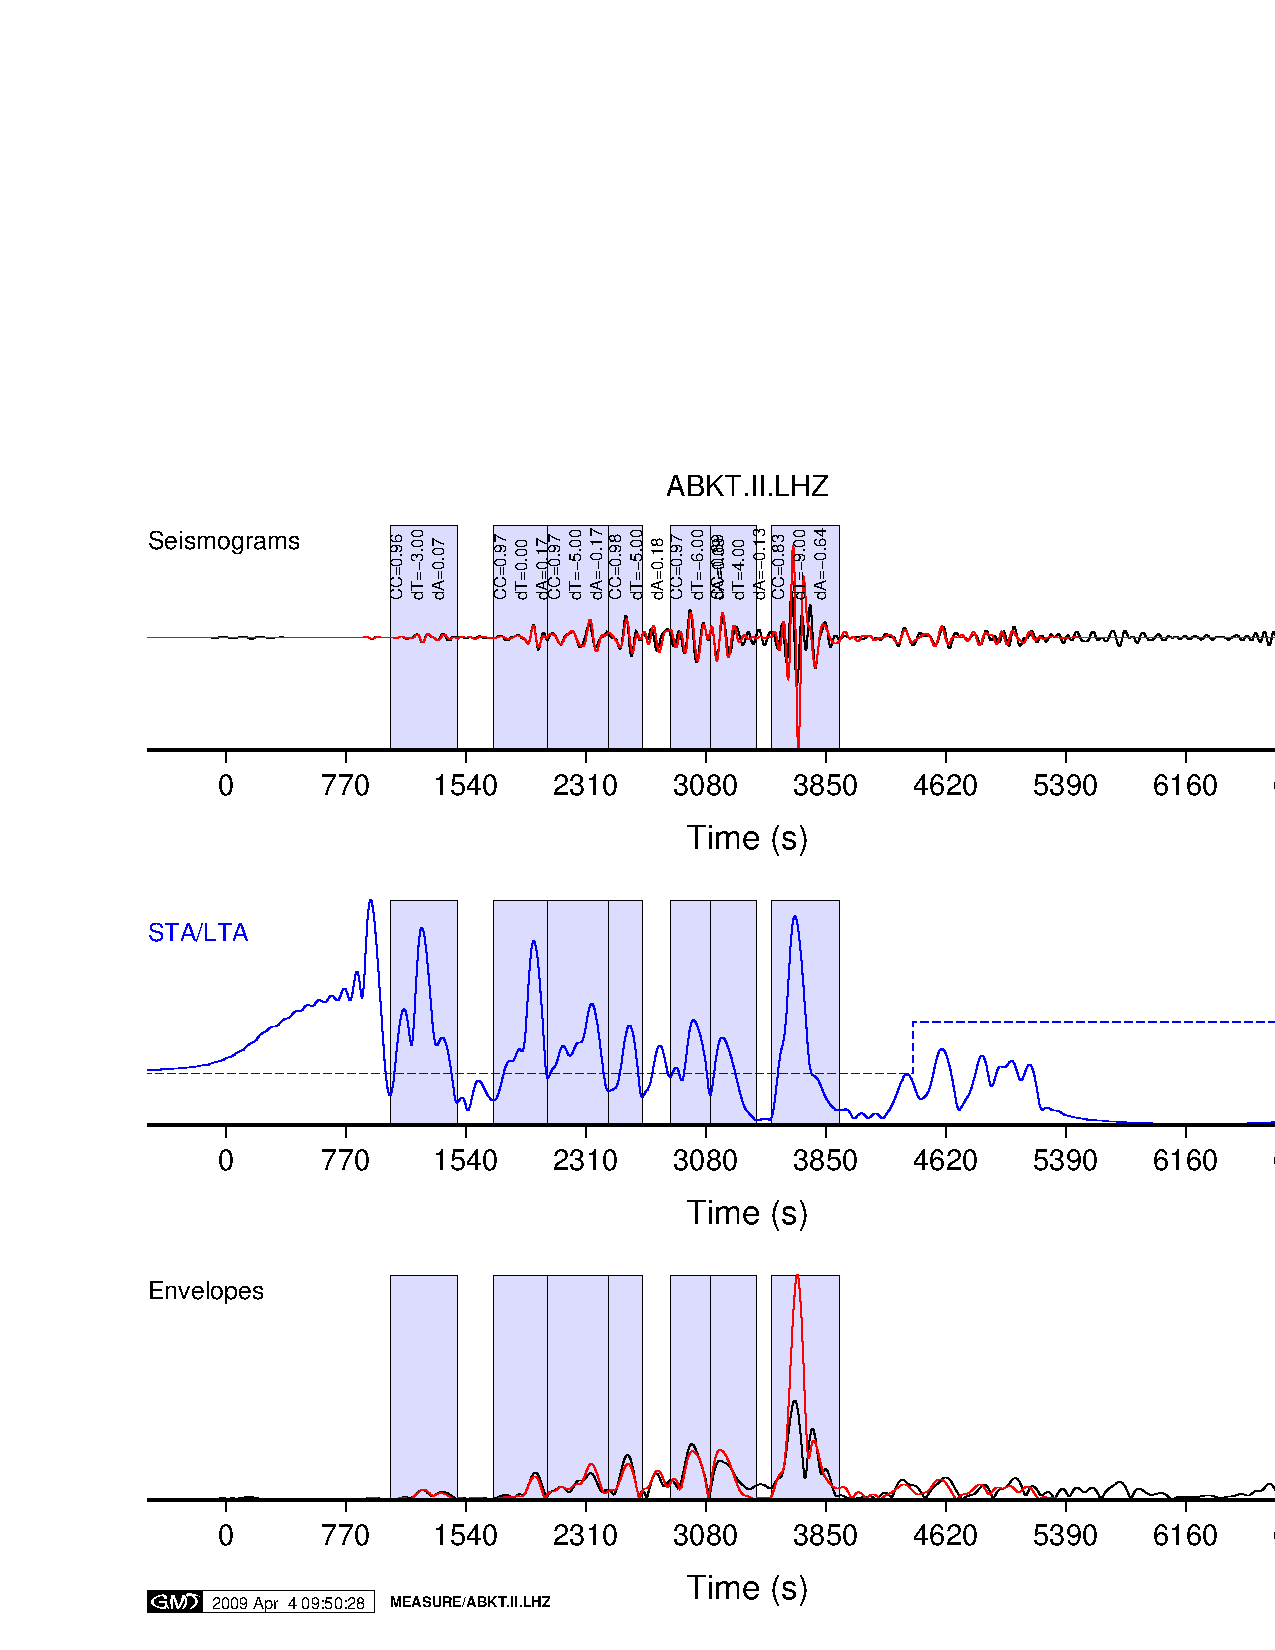
\includegraphics[width=7in]{ABKT_II_LHZ_seis.pdf}
\caption{\label{fg:test_data}
Windowing results for the test data set, plotted using the {\tt ./plot\_seismos\_gmt.sh} script.
}
\end{figure}


\section{Running FLEXWIN}

In general, flexwin is run as follows: {\tt ./flexwin < input} where the {\tt input} file is formatted as follows:
{\small
\begin{verbatim}
327
RAW_DATA/9627721.CI.ADO.BHR.sac.d.fil
SYNTH/ADO.CI.BHR.new.fil
MEASURE/ADO.CI.BHR
RAW_DATA/9627721.CI.ADO.BHT.sac.d.fil
SYNTH/ADO.CI.BHT.new.fil
MEASURE/ADO.CI.BHT
RAW_DATA/9627721.CI.ADO.BHZ.sac.d.fil
SYNTH/ADO.CI.BHZ.new.fil
MEASURE/ADO.CI.BHZ
....
\end{verbatim}
}

i.e. the number of traces to be measured, followed by (in order) the path to
the raw data sac file, the path to the synthetic sac file and the path and
basename for the (many!) output files for that trace. 

\section{Output files}
Most output files are in ascii.  All file names start with the basename given
in the input file for that trace:
\begin{description}
\item[basename.obs]	ascii observed seismogram (filtered) 
\item[basename.syn]	ascii synthetic seismogram (filtered)
\item[basename.obs\_lp.sac] sac observed seismogram (filtered)
\item[basename.syn\_lp.sac] sac synthetic seismogram (filtered)
\item[basename.env.obs]	ascii envelope of observed seismogram (filtered)
\item[basename.env.syn]	ascii envelope of synthetic seismogram (filtered)
\item[basename.win]		list of windows with theoretical phase arrival times
\item[basename.win.qual]	list of windows with Tshift,CC,dlnA values 
\item[basename.phases]		theoretical arrival times of phases
\item[basename.stalta]		STA:LTA timeseries used to select the windows, and
the time-dependent values of the STA:LTA water level, the cross-correlation
limit $CC_0$, the time-lag limit $\Delta\tau_0$, amplitude ratio limit
$\Delta\ln{A}_0$ and the window signal to noise limit $r_0$.
\item[basename.info]	information on the path and some statistics
\end{description}
For more details about the file formats, read the {\tt write\_}
subroutines in {\tt io\_subs.f90}.

\section{Scripts}
Several plotting routines ({\tt plot\_*.sh}) are provided in the {\tt scripts} subdirectory as examples for plotting seismograms, measurements and adjoint sources.  All plotting is
done using GMT (Generic Mapping Tools).  These scripts will need to be modified to suit your particular plotting needs.

The script {\tt extract\_event\_windowing\_stats.sh} extracts statistical
information on the window selection process, on the measurements.  Again,
you can use use this script as a template for your own information
extraction needs.

\section{Pre-processing suggestions}

Pre-processing is a subtle procedure that can affect the selection of windows.
Here we list some suggestions for pre-processing:
%
\begin{enumerate}
\item Interpolate raw data and ``raw'' synthetics using the same time-step.

\item Cut the data and synthetic seismograms based on the data record.  If the data record starts before the synthetic record (which is common for local earthquakes), then consider padding zeros before the synthetic record; information prior to the origin time (and P arrival) is useful in assessing the signal-to-noise ratio in the observed records.

\item Bandpass both the data and synthetics over the desired period range, rather than doing this within FLEXWIN, thereby limiting the number of filtering operations.  However, for initial determination of the bandpass range of interest, it is simpler to experiment using the FLEXWIN parameters {\tt WIN\_MIN\_PERIOD} and {\tt WIN\_MAX\_PERIOD}.
\end{enumerate}

%-------------------------------------------------
